\mysection[BrickRed]{\centering Complex Numbers}
\mysubsection{Basics}
\DEF{Def}{$\mathbb{C}=\{a+ib|a,b\in\mathbb{R}, i^2=-1\}$.}

\DEF{Def}{$z = a + ib \Leftrightarrow \Re (z)=a, Im(z)=b $}

\SA{Operations}{\begin{enumerate}
    \item $(a+ib)+(x+iy)=(a+x)+i(b+y)$
    \item $(a+ib)(x+iy)=ax+i(ay+bx)+i^2by=ax+i(ay+bx)-by=(ax-by)+i(ay+bx)$
    \item $(a+ib)(a-ib)=a^2+b^2$
    \item $\frac{a+ib}{x+iy}=\frac{(x-iy)(a+ib)}{(x-iy)(x+iy)}=\frac{(ax+by)+i(bx-ay)}{x^2+y^2}=(\frac{ax+by}{x^2+y^2})+i(\frac{bx-ay}{x^2+y^2})$
    \item $|z|=|a+ib|=\sqrt{a^2+b^2}$
    \item $\overline{a+ib}=a-ib$
    \item $|z|^2=z\overline{z}$
    \item Let $z_1,z_2\in\mathbb{C}$. Then
    \item[8a] $z_1z_2=z_2z_1$
    \item[8b] $\overline{z_1+z_2}=\overline{z_1}+\overline{z_2}$
    \item[8c] $\frac{1}{z}=\frac{\overline{z}}{|z|^2}$
\end{enumerate}}

\DEF{Euler's Formula}{Let $\theta\in\mathbb{R}$. Then $e^{i\theta}=cos\theta+isin\theta \Leftrightarrow e^{i\pi}=-1 \Leftrightarrow e^{i\pi}+1=0$.}

\DEF{Polar Coordinates}{Let $z\in\mathbb{C}$. Then $z=re^{i\theta}$ where $r\geq0$ is the modulus of $z$ and $\theta\in[0,2\pi]$ is an angle, also called the argument of $z$.}

\DEF{Fundamental Theorem of Algebra}{For any degree $n$ non-constant ($n\geq1$) polynomial $P(z)=\alpha_nz^n+a_{n-1}z^{n-1}+...+\alpha_1z+\alpha_0$ with $a_n\neq0$ $\exists \lambda\in\mathbb{C}$ s.t. $P(\lambda)=0 \Rightarrow \mathbb{C}$ is algebraically closed.}

\SA{Characteristics Polynomial}{Any degree $n$ non-constant ($n\geq1$) polynomial $P(z)=\alpha_nz^n+a_{n-1}z^{n-1}+...+\alpha_1z+\alpha_0$ with $\alpha_n\neq0$ has $n$ zeros: $\lambda_1,...,\lambda_n\in\mathbb{C}$, perhaps with repetitions, s.t. $P(z)=\alpha_n(z-\lambda_1)(z-\lambda_2)...(z-\lambda_n)$. This is called the characteristics polynomial. The number of times $\lambda\in\mathbb{C}$ appears in this expansion is called the algebraic multiplicity of the zero.}

\DEF{Hermetian Transpose}{Also called conjugate transpose. Is the natural operation of transposing for complex vectors and matrices: $A^*=\overline{A}^T=A^H$.}

\begin{figure}[H]
 \centering
 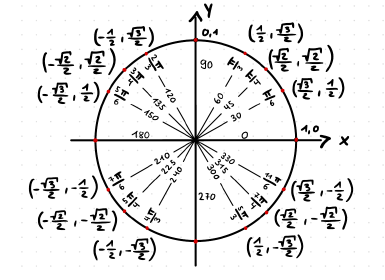
\includegraphics[width=\linewidth,keepaspectratio]{pictures/complex_numbers.png}
\end{figure}